\startchapter{Grouping For Dense Wireless Access Networks}
\label{chapter:single}

\section{Overview}


The IEEE 802.11ah standard proposed for dense sensor networks, uses a sub 1GHz band that can result in transmission ranges as high as 1 km. In a network with such a large radius and density, the traditional hidden terminal problem becomes more serious and conventional solutions do not seem to address the problem in its full extent. Recognizing this challenge, an RSS-based grouping strategy is proposed to categorize nodes in a way that the hidden terminal problem can no longer be an issue. The performance gain of the proposed method is then evaluated by an analytical model and simulations.


\section{Related Works}

\cite{tsertou2008revisiting} has considered the hidden terminal with a new approach in a Constant Contention Window (CCW) scenario and studied the problem of two competing senders that cannot sense each other but are trying to transmit to a station that both can sense, a frequent situation in infrastructure mode networks.

One solution for the hidden terminal problem is using RTS/CTS mechanism. This mechanism solves the problem for the case that the transmission time of a data packet is much larger than that of RTS/CTS. However, it introduces additional overhead, and the collisions cannot be avoided due to the RTS packets from hidden terminals. In \cite{yoonregrouping}, the hidden terminal problem in GS-DCF based networks was discussed. The proposed hidden matrix based regrouping (HMR) algorithm can reduce the number of hidden terminals but it is a centralized approach and requires the access point to discover hidden terminal relationship between two nodes first and then solve it by regrouping one of them to another group.

The research in \cite{tseng2014effective} has also studied the hidden terminal problem but in IEEE 802.15.4-based networks. A grouping mechanism similar to IEEE 802.11ah is proposed but the strategy to deal with the hidden terminal problem is still based on discovering hidden terminal relationships and rescheduling nodes.

\cite{abichar2013group} proposed a Group-based MAC where a new station join a group if the estimated distance to the group leader is below half of the transmission distance to avoid hidden-terminal, and otherwise a new group will be formed. The AP cannot effectively control the number of groups.

%The optimum way to have location based groups and solve most of potential hidden terminal problems would be the case that access point knows location information of each node and uses a clustering algorithm such as K-Means to categorize nodes in different groups and then assign each node to its designated group in way similar to centralized grouping schemes described in \cite{zheng2014performance}. 
When the AP can obtain the global information about the location of all nodes, existing clustering algorithms such as k-means can be applied and the group designation is completely controlled by the AP in a way similar to centralized grouping schemes described in \cite{zheng2014performance}.

However, when the number of terminals is large, collecting global information significantly increases the overhead of feedback. Assigning all of the nodes to their groups results in a high control overhead especially when the network is dynamic.

\section{Rss-Based Grouping Strategy}


\subsection{System Model} \label{single:systemmodel}

In this work, we consider an infrastructure based IEEE 802.11ah network, where each wireless terminal transmits its packets directly to the access point. %For simplicity, we only consider upload traffic from nodes to the access point, same as the in \cite{wu2006wsn02}. 
The network coverage area is a circle with radius $R$ where the access point is at the center. Nodes are uniformly distributed in the circle and their locations follow a Poisson Point Process (PPP) with density $\lambda$. The latter two assumptions are used for analysis and they are not necessary for the algorithm to perform. Nodes are assumed to be static at their position which is a reasonable assumption for most IoT and sensor networks and an active node always has a packet to transmit. %Active nodes are assumed to have saturated traffic. % which means every node has always a packet to transmit.

The channel model used in the analysis is a pathloss model with parameters $\alpha$ and $\beta$ in a way that the received power at a distance $d$ from the transmitter node is
\begin{equation}
P_r(d)=\frac{\beta}{d^\alpha} P_t,
\end{equation}
where $P_t$ is transmit power. In the simulation, we also consider the Rayleigh fast-fading and log-normal shadowing model where the received power is an exponential random variable and its mean $\bar{\gamma}$ is a log-normal random variable as 
\begin{equation}
\bar{\gamma}_{dB}= \mathcal{N}(10\log_{10}(P_r(d)),\sigma).
\end{equation}

%From a statistical geometric point of view, distance distribution of nodes in the same group is identical in all the schemes that are not location-based and nodes are uniformly distributed in a circle of size $A$. Therefore in this paper
We refer to both centralized and distributed schemes used in \cite{zheng2014performance} as random grouping schemes. We also do not distinguish between RAW slot crossing and not crossing cases known as CR-GS-DCF and NCR-GS-DCF respectively which has negligible impact on the grouping decision \cite{Draft80211ah}. 

\subsection{RSS-Based Grouping}
\label{rssbasedmain}
In order to avoid disadvantages of a centralized solution mentioned before, one can utilize the idea of measuring the sensed power from other nodes to let users choose their own groups based on which group their neighbors are in. Here we propose a grouping scheme based on sensed power from other nodes. % and make a comparison between them.
The grouping mechanism should be triggered by the access point (AP) using its Beacon Frame (BF) at each Grouping Update Period (GUP) and nodes should listen to the channel for the sensed power of pilot messages from group heads. Such a BF at the beginning of a GUP is called a $\text{Beacon}^\ast$ and its difference with conventional beacon frames is that there is a grouping procedure at its beginning. 



%\subsection{Semi-Centralized Average Power Based (S-CAP)}

%In the Previous schemes there is a chance that a RAW remains empty until next GUP if they no successful transmission in that RAW. In order to prevent that from happening hereWe propose a semi-centralized strategy that instead of using the average received power from conventional transmission, a node will listen to some pilot messages from randomly chosen nodes in a reserved time slot called Grouping Slot Time(GST) by an order specified by AP.
We propose an RSS-based strategy that a node will listen to some pilot messages from randomly chosen nodes in a reserved time slot called Grouping Slot Time (GST) by an order specified by the AP.

\begin{algorithm} [H]
\For{Each GUP}{
 AP chooses $M$ random nodes (group heads)\;
 AP informs group heads about their index in BF\;
 AP includes $M$ in BF\;
\For {Each node}{
\eIf {It is a group head}
{Transmits a pilot in its own GST\;}
{ Measure power of each GST\;}
}
At the end of last GST
\For {Each node}{
\eIf {It is a group head}
{Joins the group with its GST index\;}
{Joins the Group with the largest power GST index\;}
}
}
\caption{RSS-based grouping}
\end{algorithm}

A time diagram of the algorithm is illustrated in Fig. \ref{fig:diagram} and an example of Voronoi cells is shown in Fig. \ref{fig:samplevonoroli}.


\begin{figure*} [th]
  \centering
  \includegraphics[width=0.95\textwidth]{figures/diagram}
  \caption{Time diagram of RSS-based grouping algorithm, $\text{Beacon}^{\ast}$ is a BF initiating the grouping scheme. As it is shown in the figure, a GUP can be as large as several beacon intervals. Essentially it can last as long as the AP is satisfied with the throughput performance.}
  \label{fig:diagram}
\end{figure*}


%Another schemes could be the case that access point assigns $M$ random nodes to $M$ different groups and then asks them to transmit their packet in the next beacon period (or a pilot packet if they do not have any) and other nodes will choose the RAW with largest avg received power. The first $M$ group assignments will be done like the centralized method previously used in 802.11ah. 

%Just like previous scheme 
Groups are formed in Voronoi cells around group heads. Nodes will then remain in their selected RAW until another trigger from the AP.
%This scheme does not have disadvantages of above mentioned scheme but it is not as distributed as other schemes.
Comparing to centralized schemes studied in \cite{zheng2014performance} which want the AP to assign each node to a group, this scheme has a much lower control overhead and it does not require any location information to be collected and exchanged in the network.% but it has still more overhead than the aforementioned scheme (DAP).

In the rare case that a node is very far away from all the group heads, which means that it can not have any measurement for any GST, it will randomly choose one of the groups or it can report to the AP to be assigned to a group.
%In the RSS-based grouping algorithm, it is mentioned that the pilot transmissions in GST should have a higher power than usual transmissions to prevent the case that a node cannot sense a signal in any GST.
 %which is again a case that can happen in DAP algorithm. Because of such unsolved issues about the first strategy we only study performance of RSS-based grouping scheme in this paper and compare it to other random schemes and optimum solution.
 


\subsection{Implementation Issues}
The proposed scheme can be readily implemented in current IEEE 802.11 systems without any major modifications. The power measurement already exists in the MAC layer of all systems and they can provide RSSI at any time, so nodes can then find the sensed power of each GST transmission by measuring the average RSSI during the reception time of the pilot. 

GST can be as small as an ACK time and there should be some guard distance time between pilot transmissions from group heads. For the best performance, the optimum value of GUP and GST should be determined which is beyond the scope of this thesis and they do not affect our following analysis. The grouping can also be triggered by the AP if the randomly selected headers result in unsatisfactory network performance.

Including $M$ in BF is something that is already being done in the IEEE standard draft \cite{Draft80211ah}. Informing group heads about their index can also be done using a mapping strategy similar to the one used for delivery traffic indication known as DTIM.

Our algorithm is also robust against interference from other APs. Since the GSTs are short and they could be transmitted consecutively with a gap of SIFS, any other CSMA/CA based station, e.g. other APs, cannot transmit anything during the grouping procedure.

\subsection{Analytical Model}

\begin{figure} [th]
  \centering
  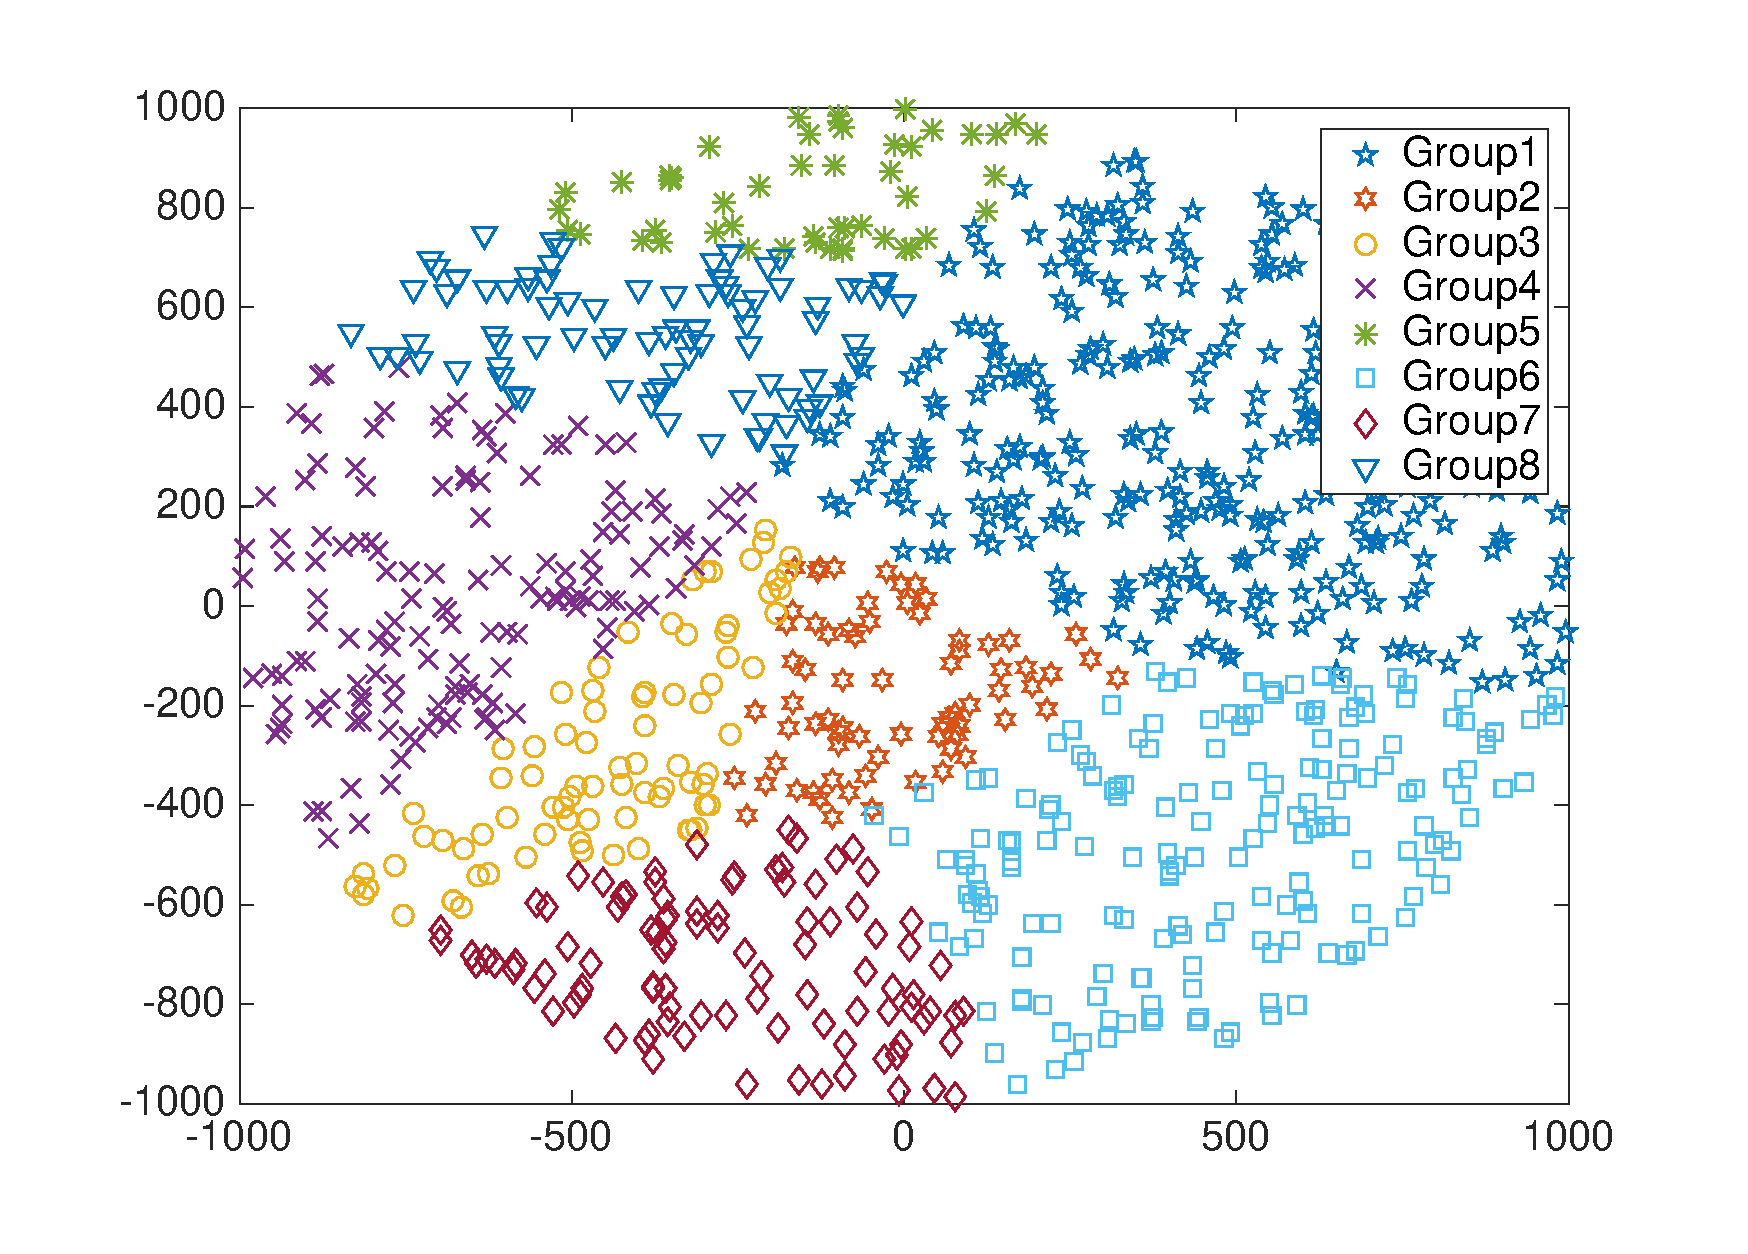
\includegraphics[width=.95\textwidth]{figures/sample_vonoroli}
  \caption{A sample grouping showing how nodes are categorized location-wise using RSS-based grouping}
  \label{fig:samplevonoroli}
\end{figure}

In order to compare the performance of grouping schemes on hidden-terminal probability, here we define two metrics and use them along with the probability of having a hidden terminal in a group to show the benefits and costs of each grouping scheme. The first metric is the average distance between nodes in a group, $D_m$, which is defined as
\begin{equation}
D_m=\frac{\sum_{i} \sum_{j \neq i} d_{ij}}{{n_m \choose 2}},  \quad \quad \forall i \text{ and } j \in \text{group $m$},
\end{equation}
where $n_m$ is the number of nodes in group $m$ and $d_{ij}$ is the distance between nodes $i$ and $j$.

The second metric is the standard deviation of the number of nodes in different groups which specifies how evenly nodes are distributed between different groups.
\begin{equation}
\sigma=\sqrt{\frac{1}{M}\sum_{m=0}^{M-1}\left( n_m - \frac{N}{M} \right)^2},
\end{equation}
where $N$ is the total number of nodes and $M$ is the number of available groups.

The next step is finding the probability of encountering the hidden terminal problem for different schemes. The number of group head nodes in our proposed strategy is fixed so their locations follow Binomial Point Process (BPP) and there are $M$ of them in the entire coverage area. Thus, the probability that there are $k$ group heads in an area of size $B$ can be found as
\begin{equation}
Pr[ N(B)=k | N(A)=M]={M \choose k} \left( \frac{B}{A} \right)^k \left( 1- \frac{B}{A} \right)^{M-k},
\end{equation}
where $A=\pi R^2$ is total area of network. We use $D$ to denote the distance between one node and its nearest group head. Every node will find its nearest group head, therefore for the CDF of $D$ we have
\begin{equation}
F_D(x)=1-Pr[N(S(x))=0 | N(A)=M] \quad x \geq 0,
\end{equation}
where $S(x)$ is the overlapping area between a circle centered at the observed node with radius $x$ and the coverage area. In general $S(x) \leq \pi x^2$ and the inequality happens for nodes close to the coverage area's border. We define $\hat{F_D(x)}$ by
\begin{equation}
\hat{F_D(x)}=1-Pr[N(\pi x^2)=0 | N(A)=M] \quad 0 \leq x \leq R.
\end{equation}
It is always true that $\hat{F_D(x)} \geq F_D(x)$ for $0 \leq x \leq R$. However, when M is large enough, which is typically the case in practice \cite{zheng2014performance} the group size is so small comparing with the whole network area that the difference between $F_D(x)$ and $\hat{F_D(x)}$ becomes negligible. We use the latter as an upper-bound of the real case.
\begin{equation} \label{eq:cdf}
\begin{split}
F_D(x) \approx \hat{F_D(x)} &=1-Pr[N(\pi x^2)=0 | N(A)=M] \\
&=1- {M \choose 0} \left( \frac{\pi x^2}{A} \right)^0 \left( 1- \frac{\pi x^2}{A} \right)^{M} \\
&=1- \left( 1- \frac{\pi x^2}{A} \right)^{M} \quad 0 \leq x \leq R.
\end{split}
\end{equation}
%The probability that $x \geq R$ is neglected in the above CDF because it is very low.
The validity of this approximation is then verified by simulation in Section \ref{single:evaluation}.

We can find PDF of $D$ by taking derivative of its CDF:
\begin{equation} \label{eq:pdf}
f_D(x)=\frac{2\pi M x}{A}(1-\frac{\pi x^2}{A})^{M-1} \quad 0 \leq x \leq R.
\end{equation}
Using this PDF we can find the probability of having a hidden terminal when our RSS-based grouping scheme is used.
\begin{figure} [th]
    \centering
    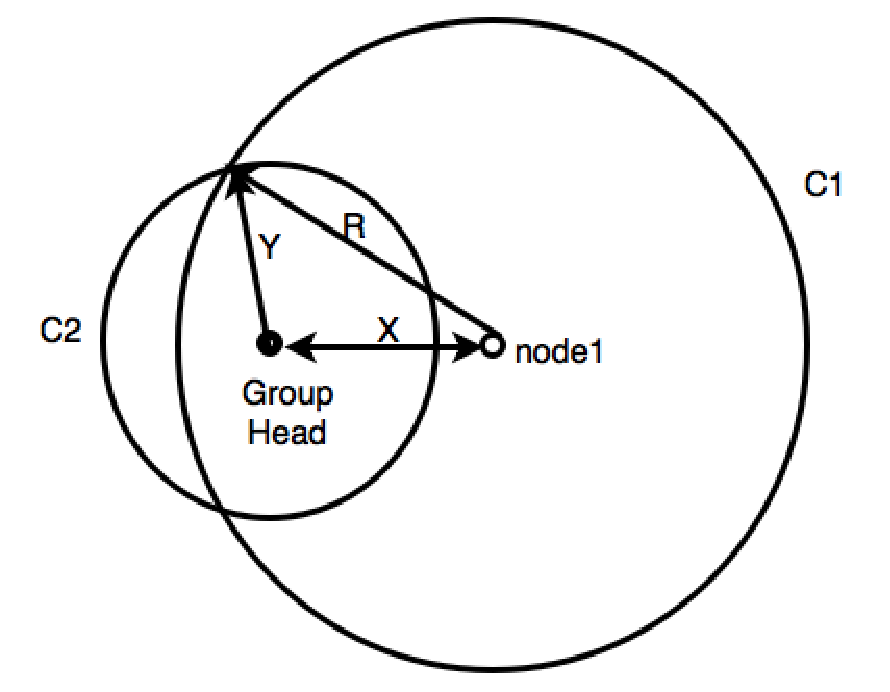
\includegraphics[width=0.75\textwidth]{figures/webb2}
    \caption{Two nodes and group head in one Voronoi cell}
    \label{fig:geometrit}
\end{figure}

Figure \ref{fig:geometrit} shows a group head and a random node called node 1 in the same group in distance $X$ where $X$ follows the PDF in (\ref{eq:pdf}). \iffalse The other node is assumed to be anywhere Within Y distance of group head. \fi The circle C1 shows the sensing range of node 1 and C2 is a circle centered by the group head with the raduis Y which also follows the PDF in (\ref{eq:pdf}). The probability for node 2 which is Y away from the group head to be in the sensing range of node 1 is the ratio of the portion of C2 inside C1 to the perimeter of C2. Then, we can take the average over the PDF of $X$ and $Y$ to obtain the probability that two nodes are within each other's sensing range.

\begin{equation}
\begin{split}
Pr_{\text{sense}}=& \\
& \int_0^{\sqrt{\frac{A}{\pi}}}\int_0^{\sqrt{\frac{A}{\pi}}} \frac{g_1(x,y)}{2\pi y} f_X(x) f_Y(y) dxdy,
\end{split}
\end{equation}
where $Pr_{\text{sense}}$ is the probability that two nodes in the same group are in each other's sensing range, $R_s$ is the sensing range of a node, 
\begin{equation}
g_1(x,y)=
\begin{cases} 
      2\pi y & R_s\geq x+y \\
      2y\arccos(\frac{x^2+y^2-R_s^2}{2xy}) & R_s< x+y \\
      0 & R_s < |x-y| 
   \end{cases},
\end{equation}
and $f_X(x)$ and $f_Y(y)$ are the PDF of $X$ and $Y$ respectively. 

We can also derive the same probability for random grouping schemes. The probability density function for the distance between two random nodes in a circle with the radius $R$ is given in \cite{moltchanov2012distance}
\begin{equation}
\begin{split}
f(r)=\frac{2r}{R^2} & \left( \frac{2}{\pi}\arccos(\frac{r}{2R}) \right. \\
& \left.  - \frac{r}{\pi R} \sqrt{1- \frac{r^2}{4R^2}} \right ) ,\quad 0<r<2R.
\end{split}
\end{equation}
In this case, for random grouping, the probability of that two nodes in the same group are in each other's sensing region can be obtained as follows,
\begin{equation}
Pr_{\text{sense}}=\int_0^{2R}g_2(r)f(r)dr,
\end{equation}
where
\begin{equation}
g_2(r)=
\begin{cases} 
      1 & r \leq R_s \\
      0 & r > R_s
   \end{cases}.
\end{equation}
These probabilities can then be calculated by numerical methods.




\section{Performance Evaluation}
\label{single:evaluation}
%The simulations used in this section are all done by MATLAB and NS-2\cite{breslau2000advances}.

%The results in this section are produced 
The performance of different grouping schemes is evaluated using MATLAB and NS-2\cite{breslau2000advances}. MATLAB is used for numerical calculations and NS-2 is used for throughput simulations. The network coverage is assumed to be a circle with radius $1$ km which is the case in sub 1GHz network having the access point at the center. As mentioned in Section \ref{single:systemmodel}, nodes are uniformly placed in the coverage area with their number following a Poisson distribution with density 0.0019 node per square meter which results in 6000 nodes in the network on average. The number of groups, M, was set in the range of 8 to 512. For each setting, the experiments were repeated 20 times, and the average was taken. 

%For each scheme the grouping is done 20 times and at each iteration an average is taken on all groups.

%We have first used our two predefined metrics to compare grouping schemes. We also calculate those metrics using a K-means clustering algorithm. 

If the AP the knows location information of all the nodes, in a pure centralized solution where AP decides the group for each node, the k-means algorithm can be used to achieve near-optimal groupings. So we can use the performance with k-means grouping as a benchmark to see how well our RSS-based distributed grouping algorithm is working compared with the centralized benchmark.

In Fig. \ref{fig:meansum}, the average distance between nodes in a group for the proposed scheme is always smaller than with the random grouping scheme and close to the k-means clustering algorithm. It is also obvious that a larger number of groups have a smaller average distance between nodes for all algorithms. 

In Fig. \ref{fig:variance}, we can see that the standard deviation of the number of nodes in different groups is the cost that the RSS-based grouping algorithm pays for the advantage of distributed solution. Groups with a large number of users will suffer from high collision probability and groups with a very small number of users may not fully utilize their RAW. It is shown later using NS-2 simulations, that despite having some dense groups, the RSS-based grouping algorithm has a better performance than random groupings. This is because the hidden node problem is a more severe problem than uneven groups. A few hidden terminals can dramatically decrease the performance of the whole network. Having more nodes that are all in the sensing range increases the competition but has a less destructive effect on the throughput than that due to hidden terminal.



\begin{figure} [th]
  \centering
  \subfloat[][Average $D_m$ over all groups]{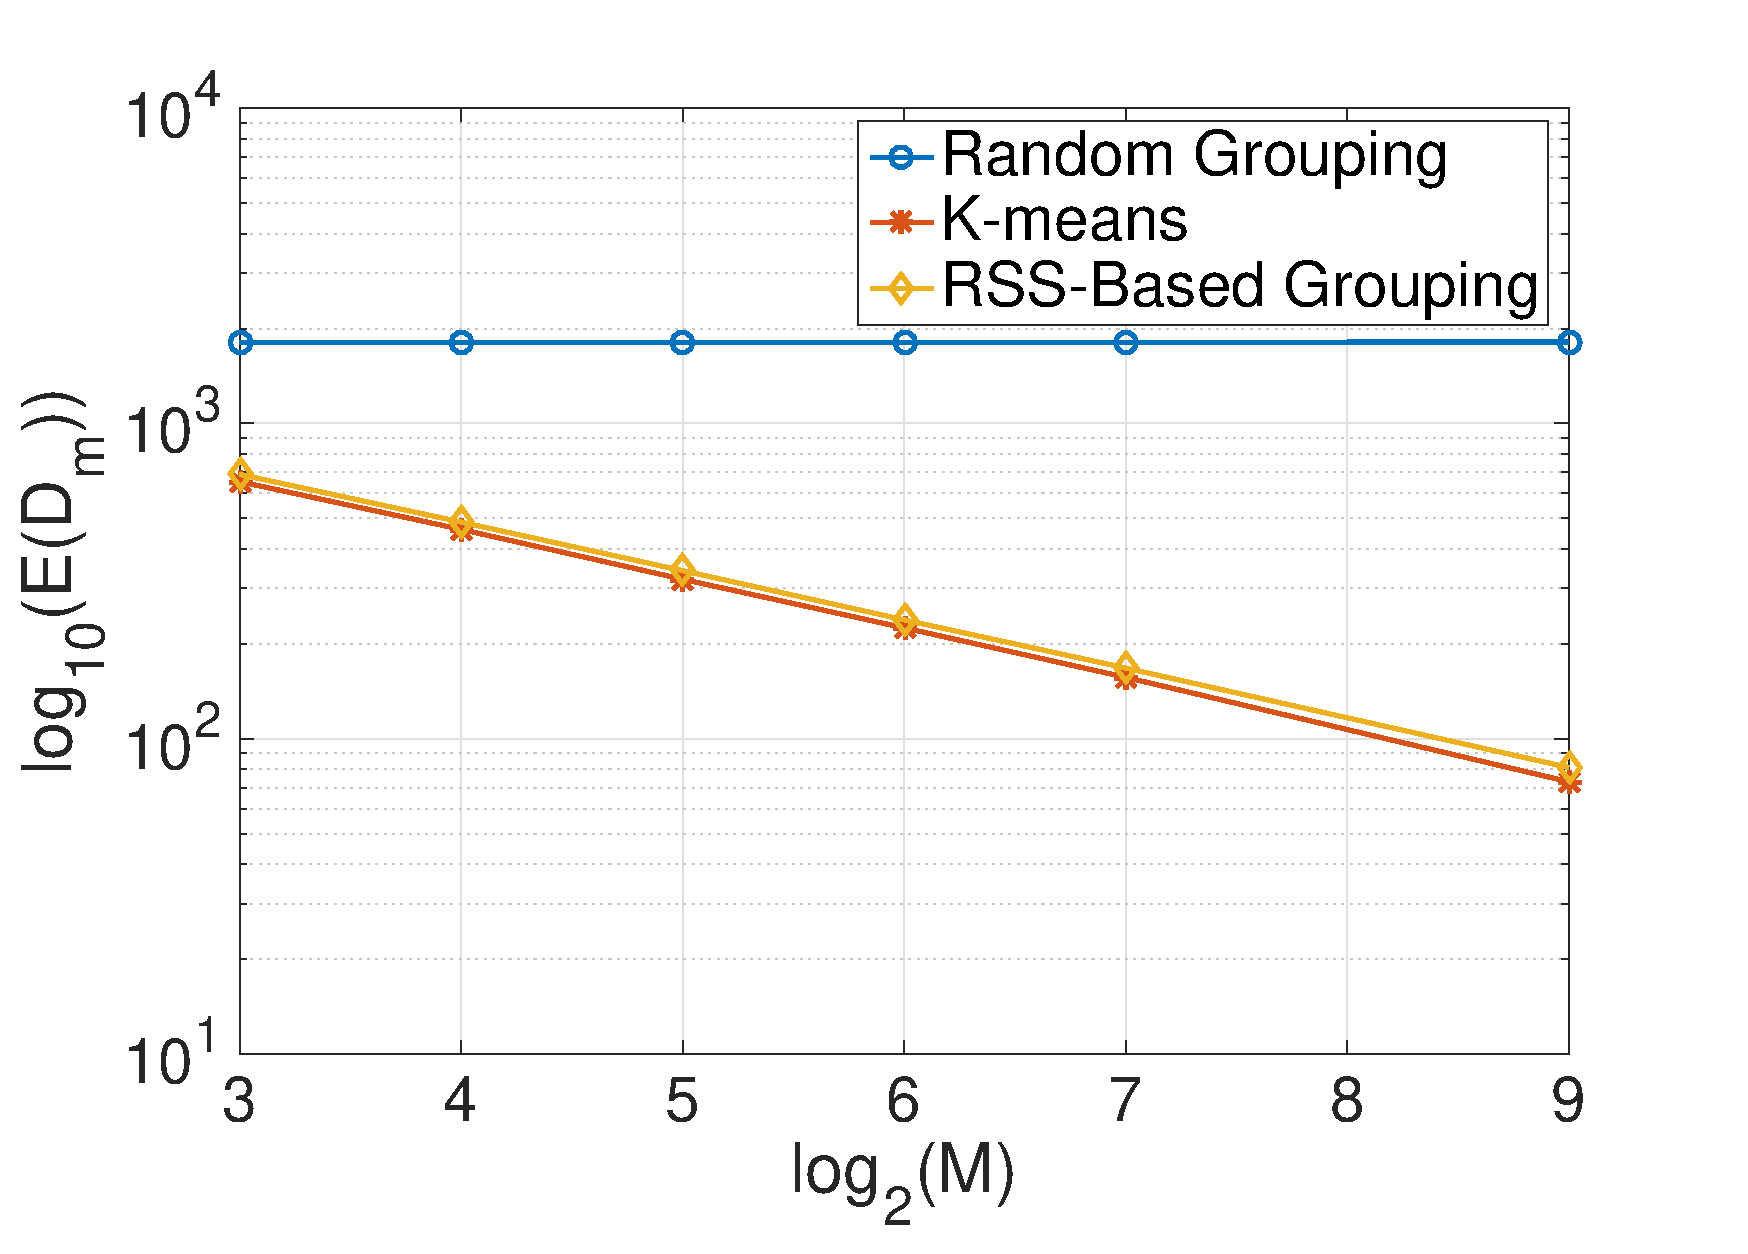
\includegraphics[width=.5\textwidth]{figures/final_metric1}%
  \label{fig:meansum}}
  \subfloat[][Standard deviation of the number of nodes in different groups]{\includegraphics[width=.5\textwidth]{figures/final_metric2}%
  \label{fig:variance}}
  \caption{Grouping performance metrics}
  \label{fig:metricx}
\end{figure}

\iffalse
\begin{figure} [th] 
  \centering
  \includegraphics[width=.95\textwidth]{figures/final_metric2}
  \caption{Simulation result for standard deviation of the number of nodes in different groups}
  \label{fig:didi}
\end{figure}
\fi

%Considering the higher transmission power and the receiving antenna gain at the AP side, we assume that the sensing distance between two user nodes may be equal to or smaller than the maximum transmission distance to the AP.
Assuming that all nodes have the same sensing range, $R_s$, the probability of two random nodes in the same group be in their sensing range versus $R_s$ for a constant number of groups is shown in Fig. \ref{fig:prob}. The figure also shows that the approximation in (\ref{eq:cdf}) not affect the result very much. As we can see in the figure, best performance is for the clustering using the k-means algorithm but the RSS-based grouping scheme also performs very close to the k-means and much better than the random grouping schemes. The same probability assuming Rayleigh fading channel between nodes is also shown in Fig. \ref{fig:prob}. The performance with Rayleigh fading channels is degraded because considering fast fading the areas occupied by groups are no longer Voronoi and the group head with the highest sensed power is not necessarily the closest one. As shown in the figure the algorithm still performs well which indicates that, the RSS estimation accuracy required is low, which results in a small overhead.

With the simulation results following analytical results, our assumption in section \ref{single:systemmodel} is verified. The simulation and analytical results are closer to each other as M grows. That is because, with a higher value of M, the edge effect becomes more negligible.

%the probability that a node's distance to its group head is larger that R becomes smaller.
%Probability of having hidden terminal versus number of group for a constant range ,for avg-power based and random grouping schemes is shown in figure \ref{fig:prob2}

\begin{figure} [th]
  \centering
  \subfloat[][]{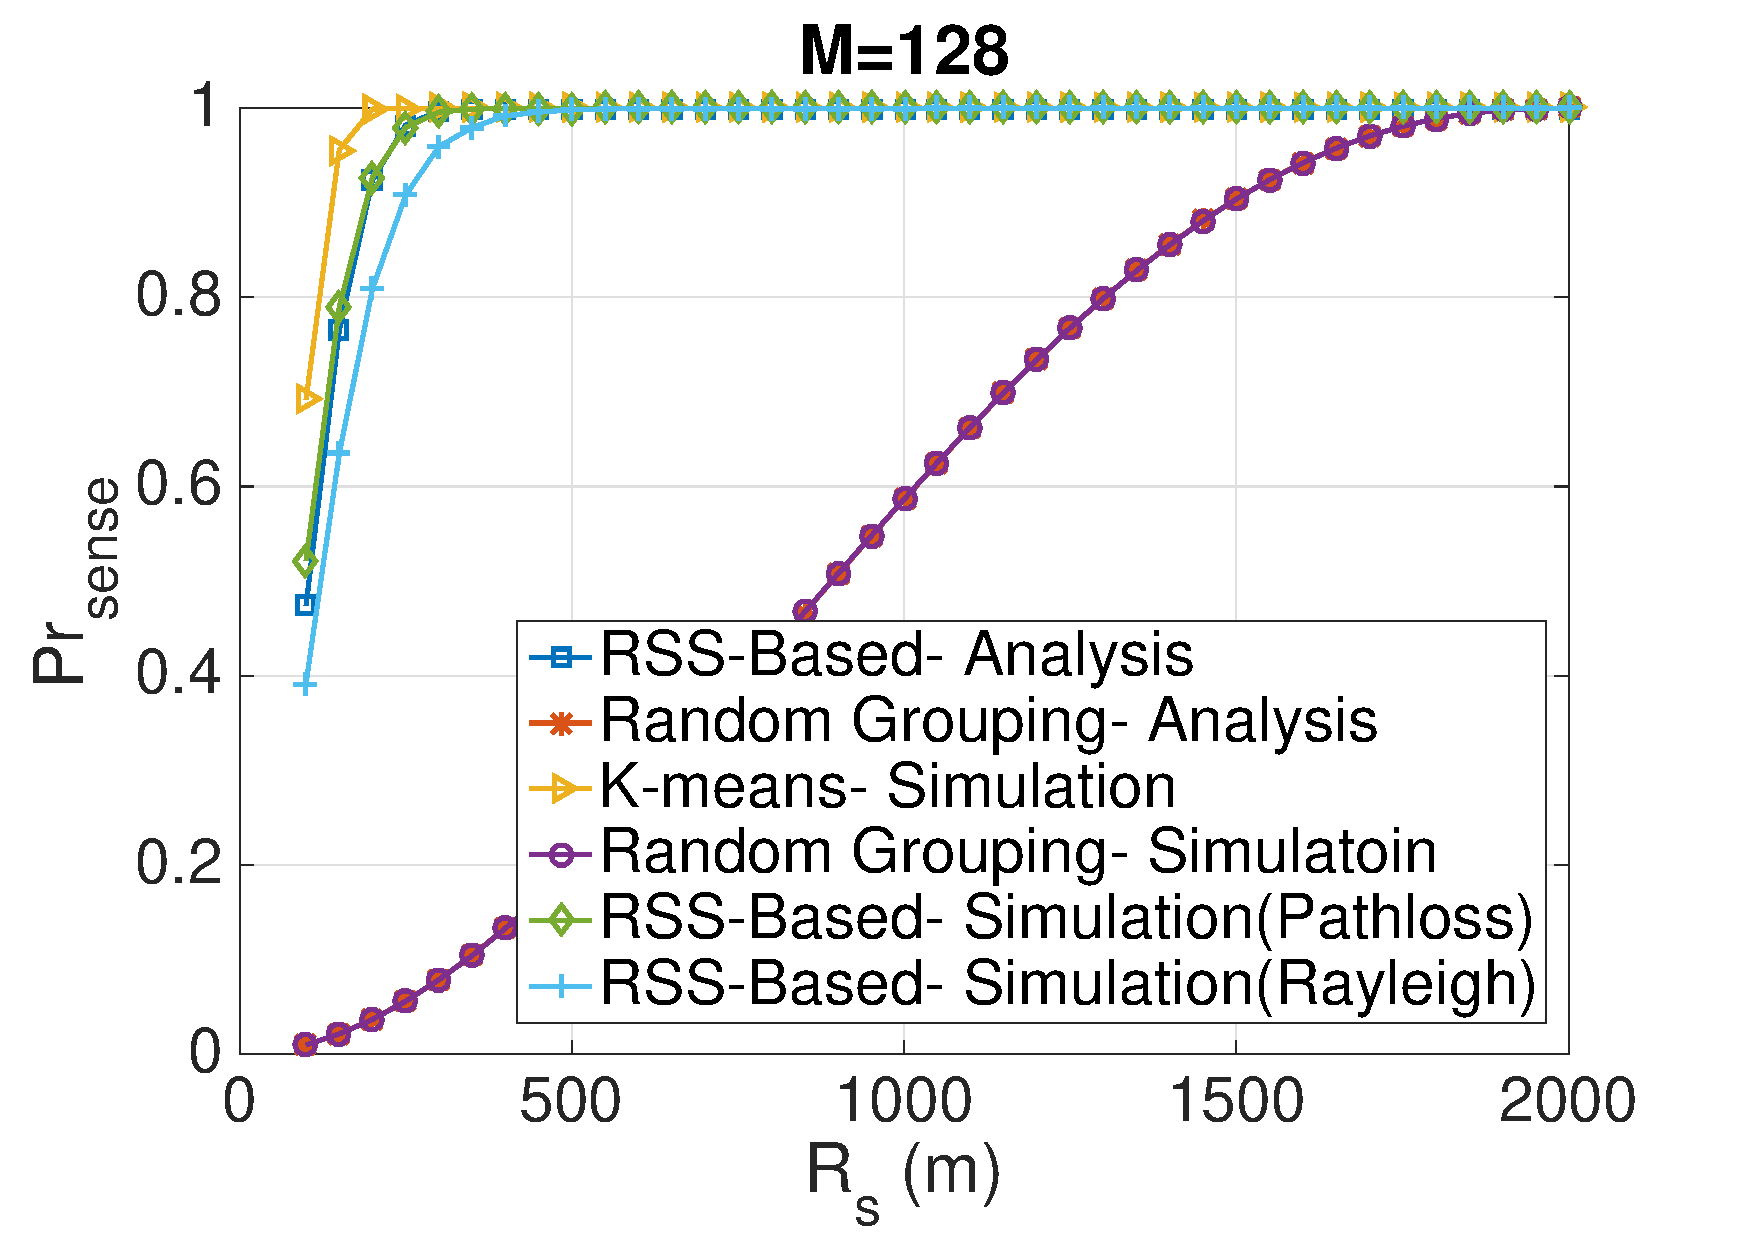
\includegraphics[width=.47\textwidth]{figures/final_probability_fixedM}%
  \label{fig:prob}}
  \subfloat[][]{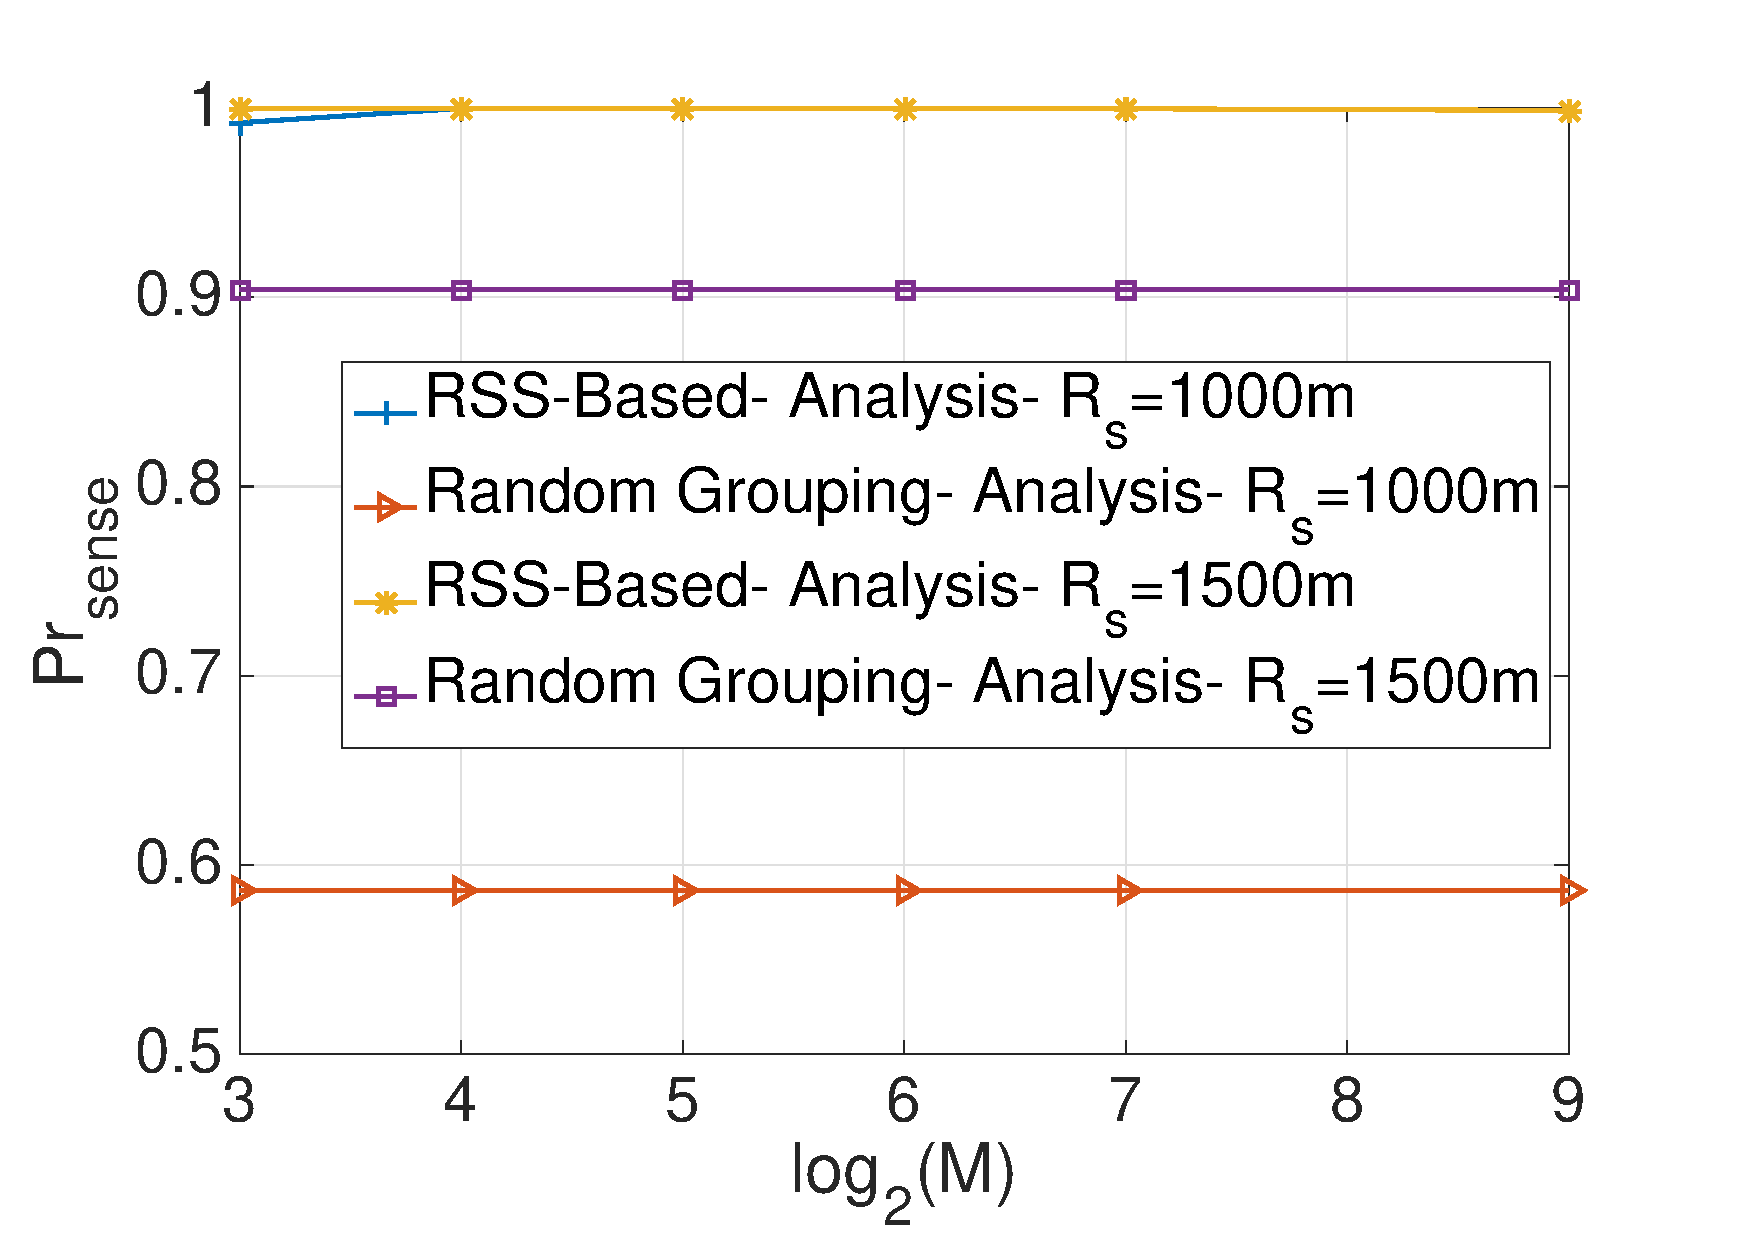
\includegraphics[width=.47\textwidth]{figures/final_probablity_fixedR_analysis}%
  \label{fig:prob2}}
  \caption{Probability of two nodes, within a group, being in the sensing range of each other}
  \label{fig:probabilities}
\end{figure}


\iffalse
\begin{figure} [th]
  \centering
  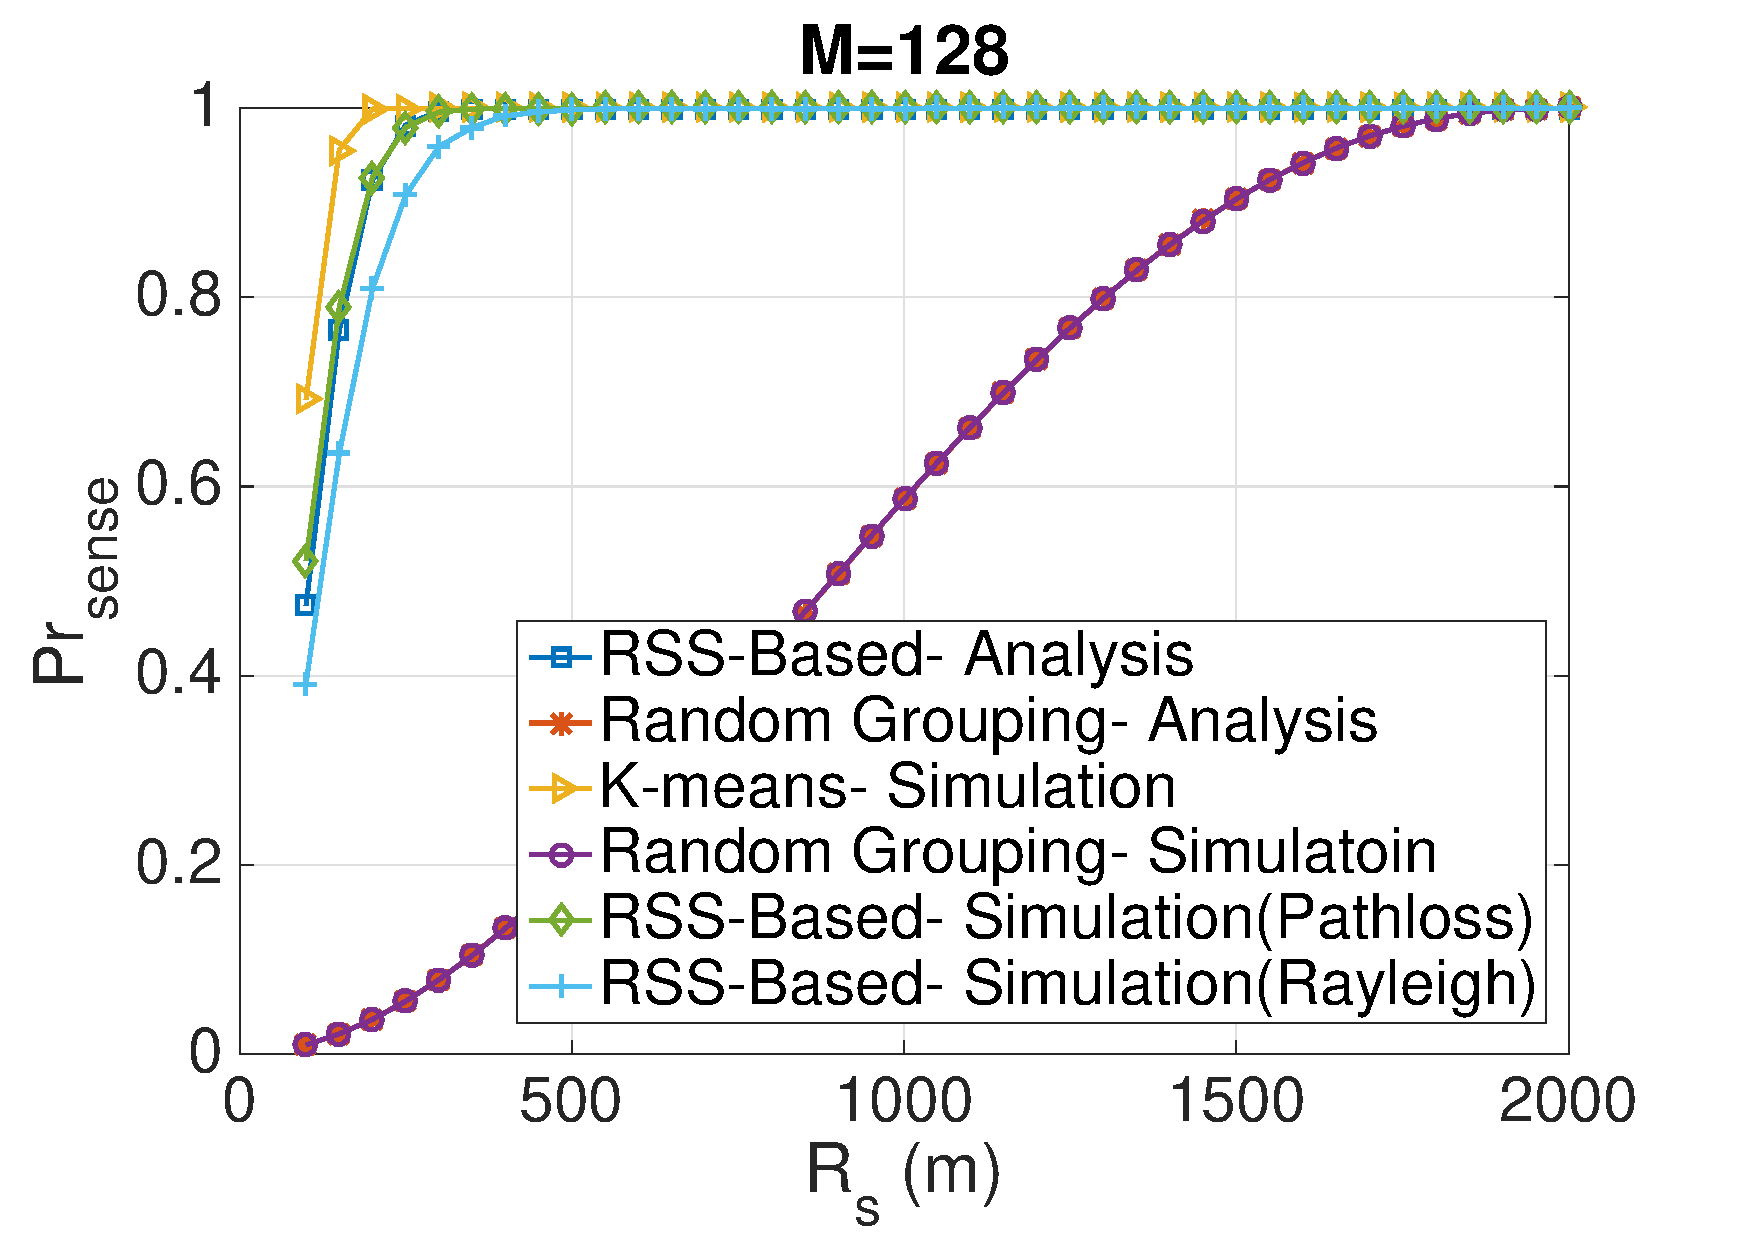
\includegraphics[width=.95\textwidth]{figures/final_probability_fixedM}
  \caption{Probability of two nodes, within a group, in the sensing range of each other}
  \label{fig:prob}
\end{figure}
\fi
Fig. \ref{fig:prob2} shows the probability of two nodes in the same group being in each other's sensing range when all nodes' sensing range is fixed and the number of groups changes. This probability does not change with the number of groups for random grouping because nodes in the same group can still be anywhere in the coverage area and their distance still follows the same PDF. Though in case of the RSS-based grouping algorithm, a larger number of groups results in a higher probability for group members to be in the sensing range of each other because it makes the Voronoi cells smaller.    

\iffalse
\begin{figure} [th]
  \centering
  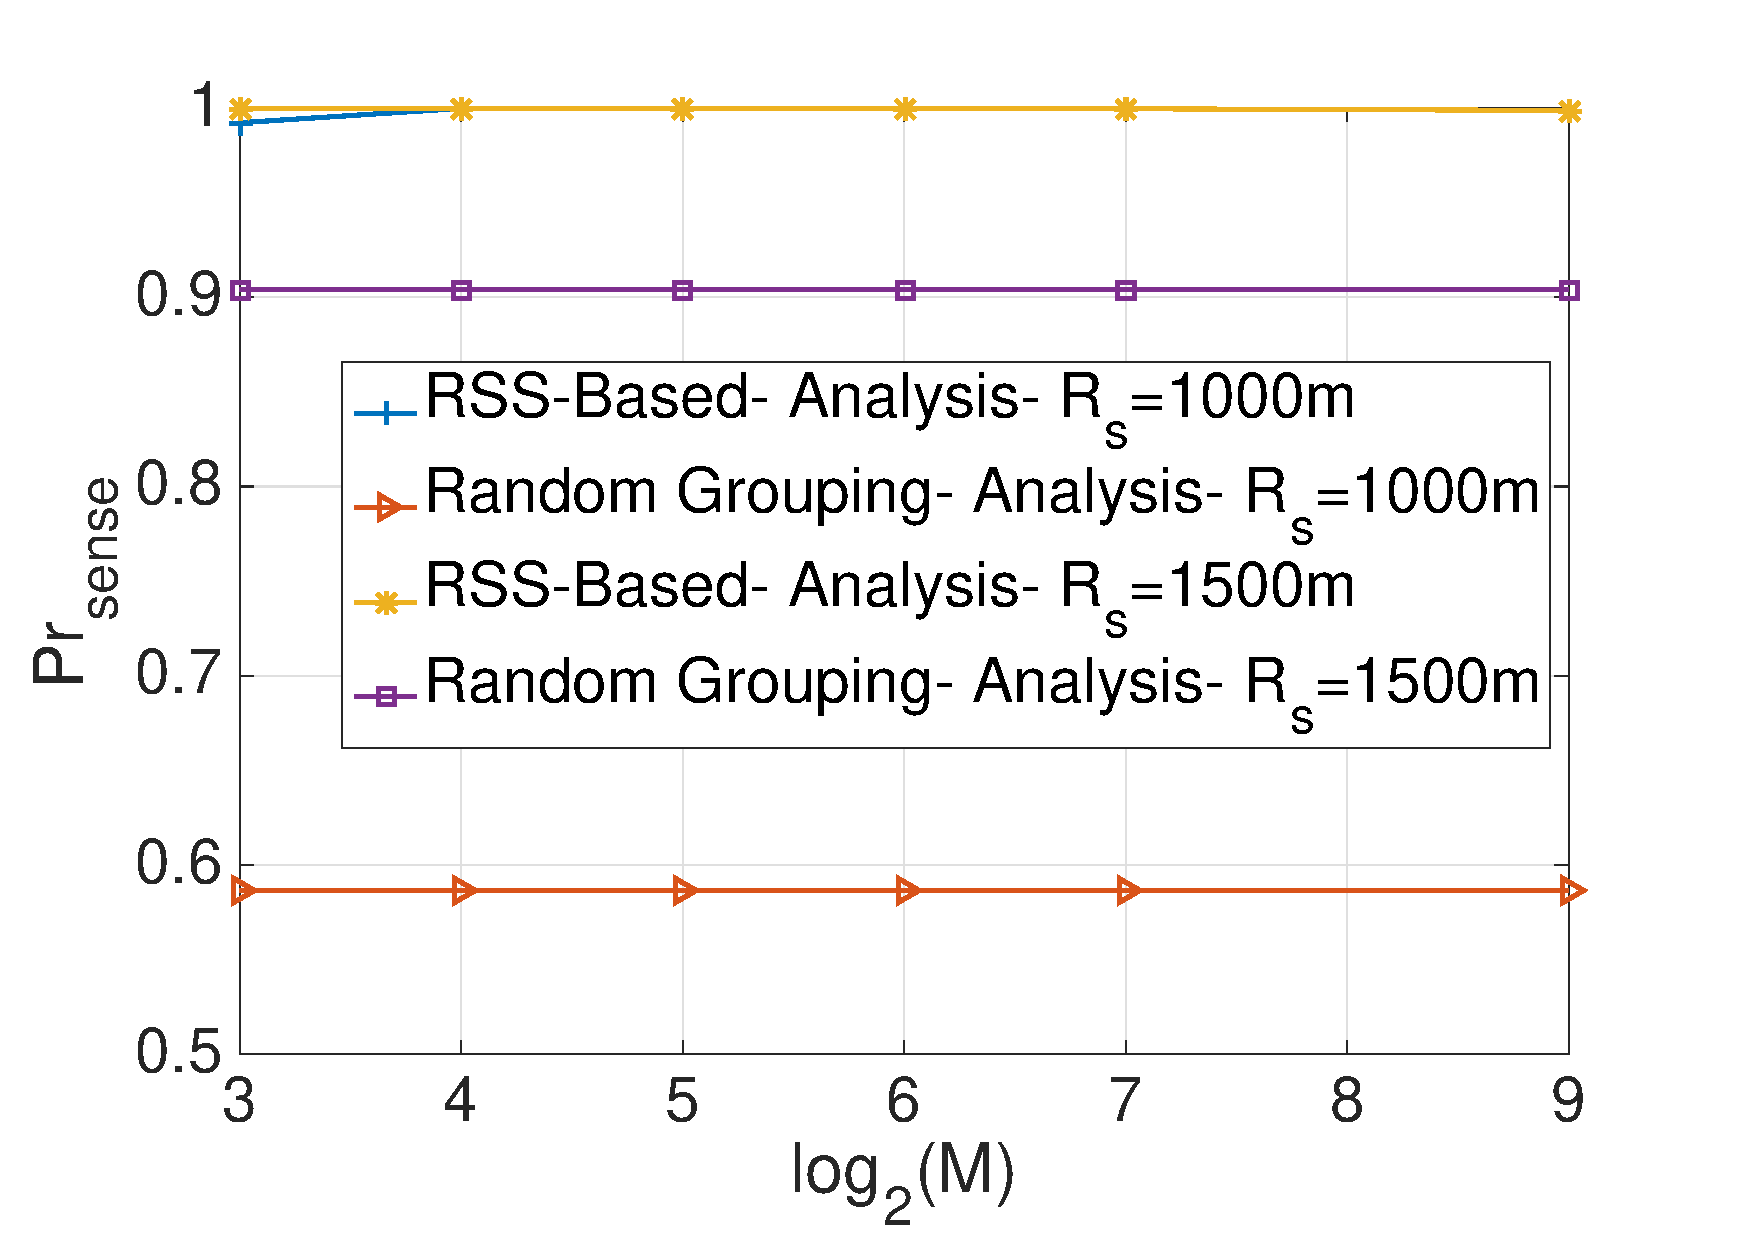
\includegraphics[width=.95\textwidth]{figures/final_probablity_fixedR_analysis}
  \caption{Probability of two nodes, within a group, in the sensing range of each other}
  \label{fig:prob2}
\end{figure}
\fi

Fig. \ref{fig:throughput} shows the throughput simulation result for different grouping schemes along with k-means clustering algorithm using NS-2. Table \ref{table:throughput} shows the parameter setting for simulations used in this section. Other common settings such as PHY and MAC header are set according to the IEEE 802.11 standard \cite{wlan2011}. The payload size is set to be low considering the IoT applications such as smart meter measurement reporting and all nodes are using RTS/CTS mechanism. Only the uplink traffic is considered and a non-collided transmission is assumed to be successful which that means the PHY layer BER is not considered. 

\begin{figure} [th] 
  \centering
  \includegraphics[width=.95\textwidth]{figures/throughput}
  \caption{Throughput of Uplink traffic}
  \label{fig:throughput}
\end{figure}

 In Fig. \ref{fig:throughput}, the throughput for random scheme is very low because the time for a single packet transmission is more than the largest back off window (1024 slots) and almost any transmission would be interrupted when there is a few active nodes who are hidden terminals. In other words, \iffalse in a saturated traffic scenario, \fi a node with a hidden terminal may hardly success in transmitting a packet to the AP without collision.

This figure also shows the limited cost that RSS-based grouping pays due to the higher standard deviation of number of nodes in each group. The throughput using the proposed RSS-based grouping is close to that using the centralized K-mean solution. On the other hand, random grouping has much worse performance due to the hidden terminal problem even when the sensing range is as high as 1500m. Note that the theoretical sensing range without considering the shadowing effect may be much higher than the practical sensing range, so grouping considering the location is important to avoid hidden terminal and improve network performance.


\begin{table}
% increase table row spacing, adjust to taste
%\renewcommand{\arraystretch}{1.3}
%if using array.sty, it might be a good idea to tweak the value of
%\extrarowheight as needed to properly center the text within the cells
\caption{Throughput Simulation Parameter Setting}
\label{table:throughput}
\centering
% Some packages, such as MDW tools, offer better commands for making tables
% than the plain LaTeX2e tabular which is used here.
\begin{tabular}{|c||c|}
\hline
Parameter & Value \\  
\hline
 Slot time & 20 $\mu$S \\ 
 \hline
 SIFS & 10 $\mu$S \\
 \hline
 Payload Size & 64 bytes\\ 
\hline
Data Rate & 1Mbps \\
\hline
$R_s$ & 1500 \\
\hline 
CW min & 31 \\
\hline
CW max & 1023 \\
\hline 
\end{tabular}
\end{table}